
\section{Results}
\label{sec:results}

The results for each feature selection model were somewhat unexpected, in that the basic model exceeded expectations. Table 2 shows the F1 scores for each model. Unsurprisingly, KNN outperforms the logistic regression for every feature selection method, as predicted. This makes sense given the complexity of the problem and the large number of features. However, the basic model outperformed the Canny model, meaning that the features of the clothing beyond just the shape was important to correctly classifying it. This also makes sense given the complexity of the problem, meaning removing features means less of the complexity is captured and biasing the model more.

\begin{table}[!h]
    \centering
    Cross Validation Results\\
    \begin{tabular}{|l|c c c|}
    \hline
         Model & Basic & Canny & Combined\\
         \hline
         Baseline & 0.018 & 0.018 & 0.018\\
         Logistic Regression & 0.783 & 0.692 & 0.783\\
         KNN & 0.856 & 0.804 & 0.855\\
         \hline
    \end{tabular}
    \caption{F1 scores for cross validation test data}
    \label{tab:my_label}
\end{table}

However, the most unexpected result was that the combined model performed equally as well as the basic model. Our guess is that the distances between color values on the basic half were much larger, giving those features a much heavier weight. This makes sense as the performance difference between both feature selection methods is essentially negligible.

Since the KNN models consistently outperformed the logistic regression models, we included confusion matrices only for the KNN models to better understand where they were making incorrect predictions. As can be seen in figures 8, 9, and 10, for all models, as predicted, the largest sources of error was mixing up the "T-shirt/top" and "Shirt" labels, and the "Coat" and "Pullover" labels. Additionally,  the "Shirt" and "Pullover" labels and the "Sneaker" and "Sandal" labels were also sources of error. This is still promising, as the model is mainly confusing similar articles of clothing rather then, for example, confusing shoes and shirts. Both the basic and combined feature selection methods had similar error distribution among categories, which further corroborates our theory above.

\begin{figure}[!h]
    \centering
    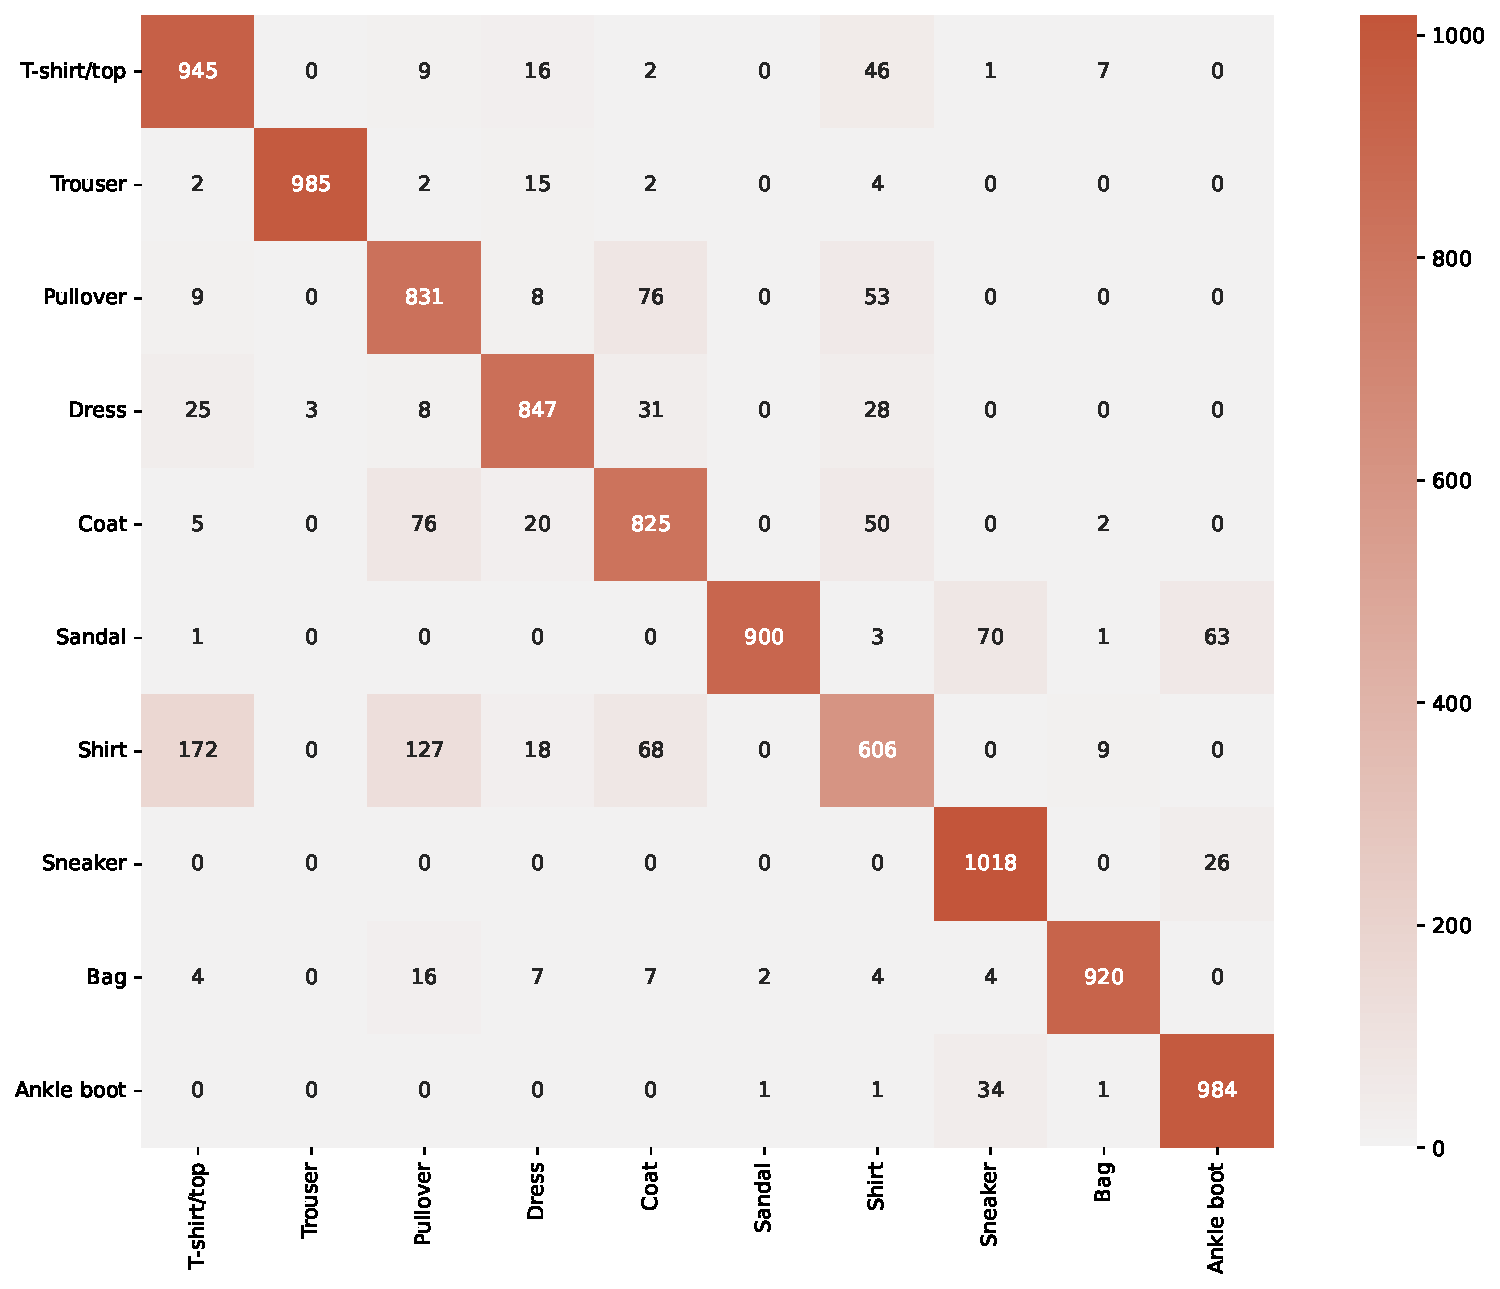
\includegraphics[width=3.5in]{basic_knn_cmatrix.pdf}
    \caption{Confusion Matrix for the basic model, predicted labels are the rows and actual labels are the columns}
    \label{fig:my_label}
\end{figure}

\begin{figure}[!h]
    \centering
    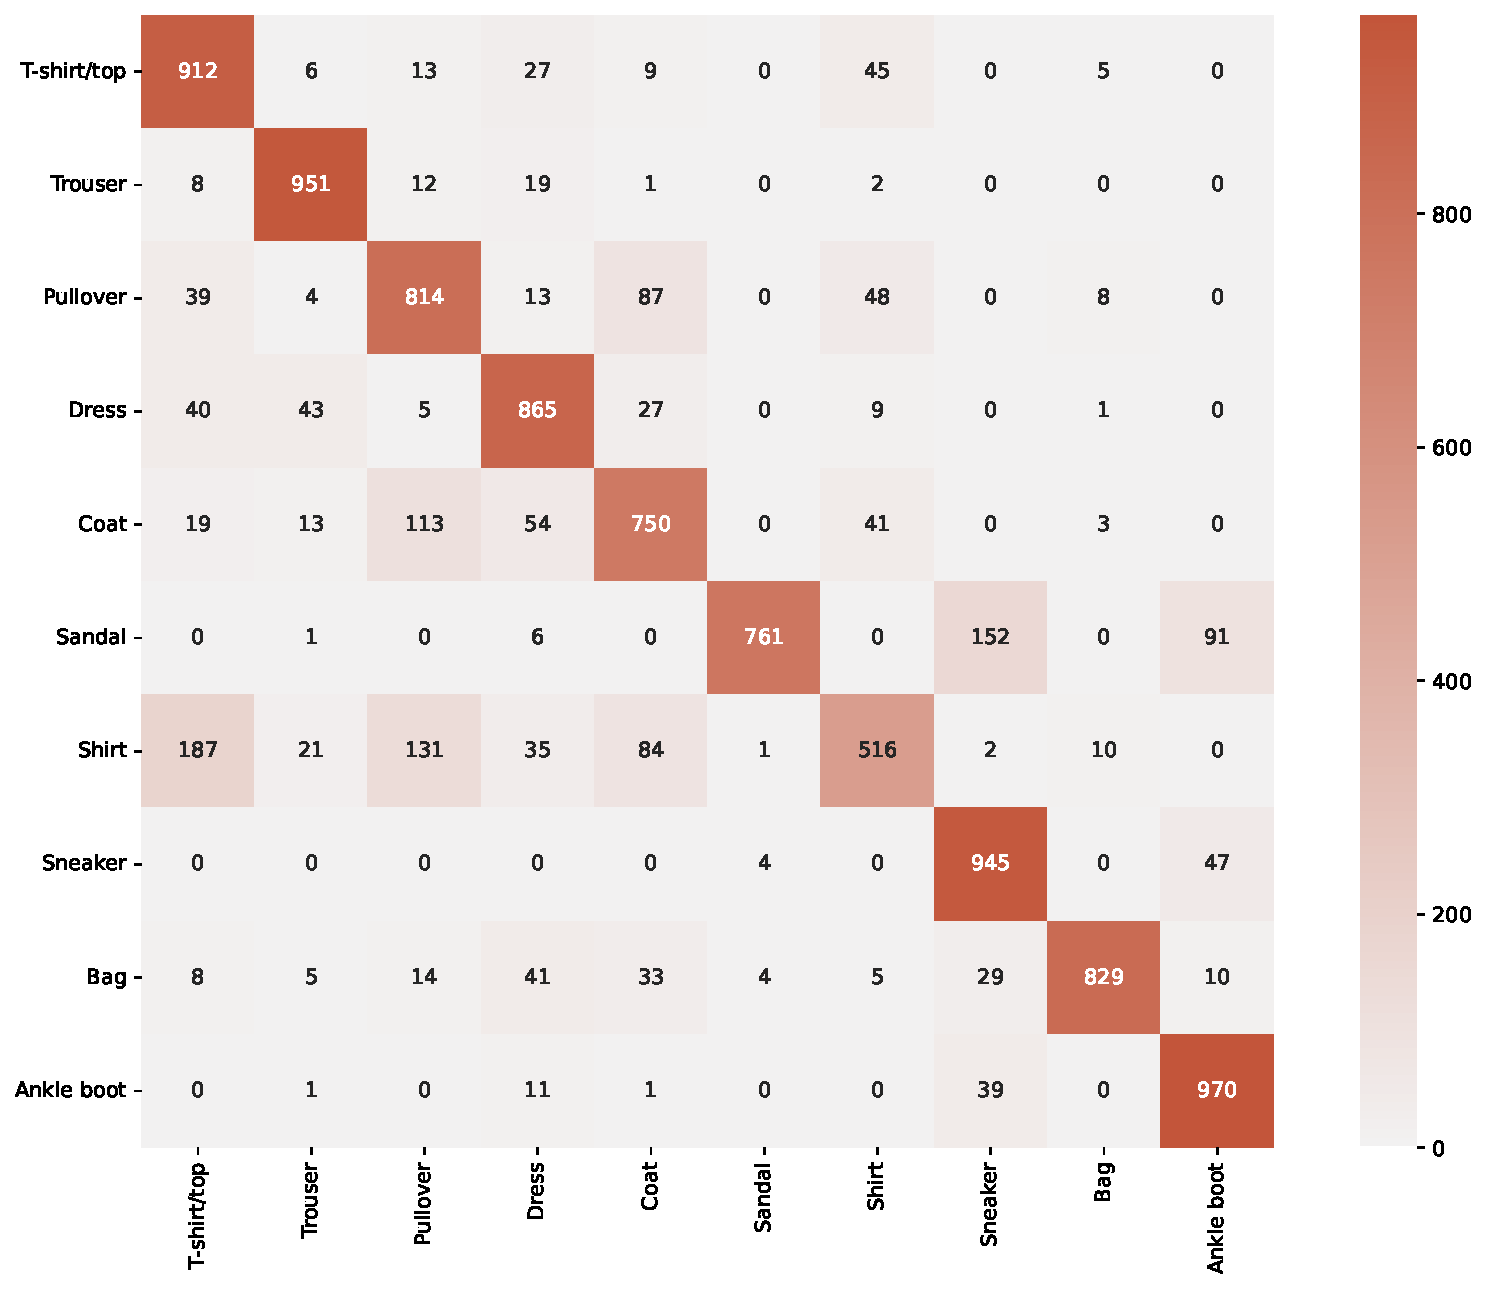
\includegraphics[width=3.5in]{canny_knn_cmatrix.pdf}
    \caption{Confusion Matrix for the Canny model, predicted labels are the rows and actual labels are the columns}
    \label{fig:my_label}
\end{figure}

\begin{figure}[!h]
    \centering
    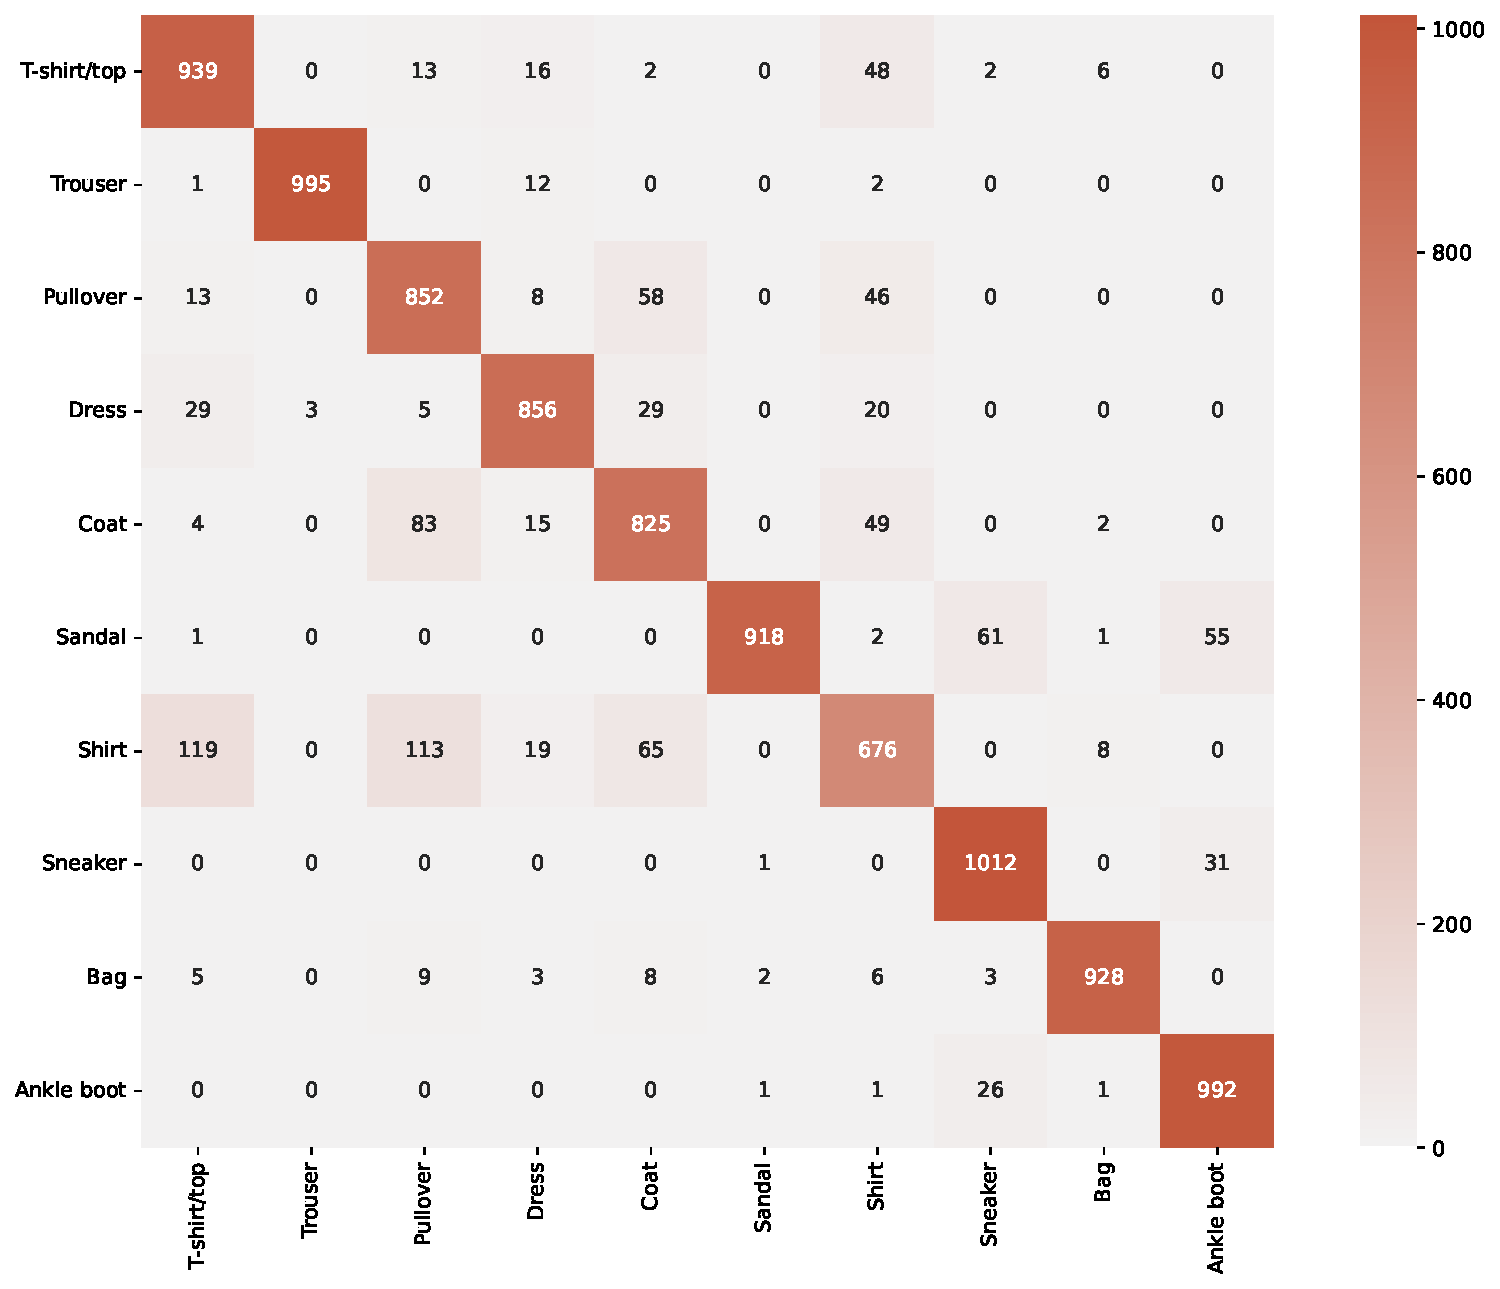
\includegraphics[width=3.5in]{combined_knn_cmatrix.pdf}
    \caption{Confusion Matrix for the combined model, predicted labels are the rows and actual labels are the columns}
    \label{fig:my_label}
\end{figure}


After tuning hyper-parameters and running the cross-validation tests, we tested the model on the final test data to get an estimate for accuracy with unseen data to see if our models overfit our training data. As displayed in table 3, most of the final test results are the same (or very similar) as the cross-validation test results-meaning the models had low variance. However, the final test score for the combined KNN model was identical to the cross-validation score, however the basic KNN model was slightly worse on the final testing data. 

\begin{table}[!h]
    \begin{center}
        Final Test Results\\
    \begin{tabular}{|l|c c c|}
    \hline
         Model & Basic & Canny & Combined\\
         \hline
         Baseline & 0.018 & 0.018 & 0.018\\
         Logistic Regression & 0.774 & 0.678 & 0.774\\
         KNN & 0.852 & 0.801 & 0.855\\
         \hline
    \end{tabular}
    \caption{F1 scores for final test data}
    \label{tab:my_label}
    \end{center}
\end{table}

This leads us to believe that the edge detection is \textit{slightly} useful in classifying clothing, as long as it is not done in isolation. Even though both the basic and combined models fit the testing data similarly, the extra edge detection features seem to create a more generally reliable model. However, the difference in F1 score of 0.003 is so slim that it is essentially negligible.

Our models all significantly outperformed our baseline model, and our KNN models even outperformed the Bossard et al. random forest model for all metrics. However, the Zhou et al. paper's use of neural networks seems to be the best approach, as their 0.93 F1 score is impressively accurate. Even though we technically outperformed the Bossard et al. paper, both papers performed the classification on images with noisy backgrounds and color, requiring more advanced feature selection techniques to isolate the important information in each image. However, for this more simplistic version of clothing classification, our model would still be useful in providing a first labeling of each article in a controlled environment, even if humans would be needed to double check images and relabel any errors.





